\documentclass[10pt,a4paper]{article}

% Set the page margins.
\usepackage[a4paper,margin=0.75in]{geometry}
\usepackage{graphicx}
\graphicspath{ {images/} }

% Setup the language.
\usepackage[english]{babel}
\hyphenation{Some-long-word}

% Makes resume-specific commands available.
\usepackage{resume}

\newcommand*{\plogo}{\fbox{$\mathcal{PL}$}} % Generic logo

%----------------------------------------------------------------------------------------
%	TITLE PAGE
%----------------------------------------------------------------------------------------

\newcommand*{\titleGP}{\begingroup % Create the command for including the title page in the document
\centering % Center all text
\vspace*{\baselineskip} % White space at the top of the page

\rule{\textwidth}{1.6pt}\vspace*{-\baselineskip}\vspace*{2pt} % Thick horizontal line
\rule{\textwidth}{0.4pt}\\[\baselineskip] % Thin horizontal line

{\LARGE Ironman Image Throw Thingy\\ by \\[0.3\baselineskip] CSIR}\\[0.2\baselineskip] % Title

\rule{\textwidth}{0.4pt}\vspace*{-\baselineskip}\vspace{3.2pt} % Thin horizontal line
\rule{\textwidth}{1.6pt}\\[\baselineskip] % Thick horizontal line

\scshape % Small caps
A tender document for the consideration of the\\ % Tagline(s) or further description
CSIR Ironman Image Throw Thingy Project \\[\baselineskip] % Tagline(s) or further description
4 May 2015\par % Location and year

\vspace*{2\baselineskip} % Whitespace between location/year and editors

Edited by \\[\baselineskip]
{\Large Werner Mostert \\ Keagan Thompson \\ Kale-ab Tessera \\ Michelle Swanepoel 
\\ Abrie van Aardt
\par} % Editor list
\vspace*{2\baselineskip}
\fbox{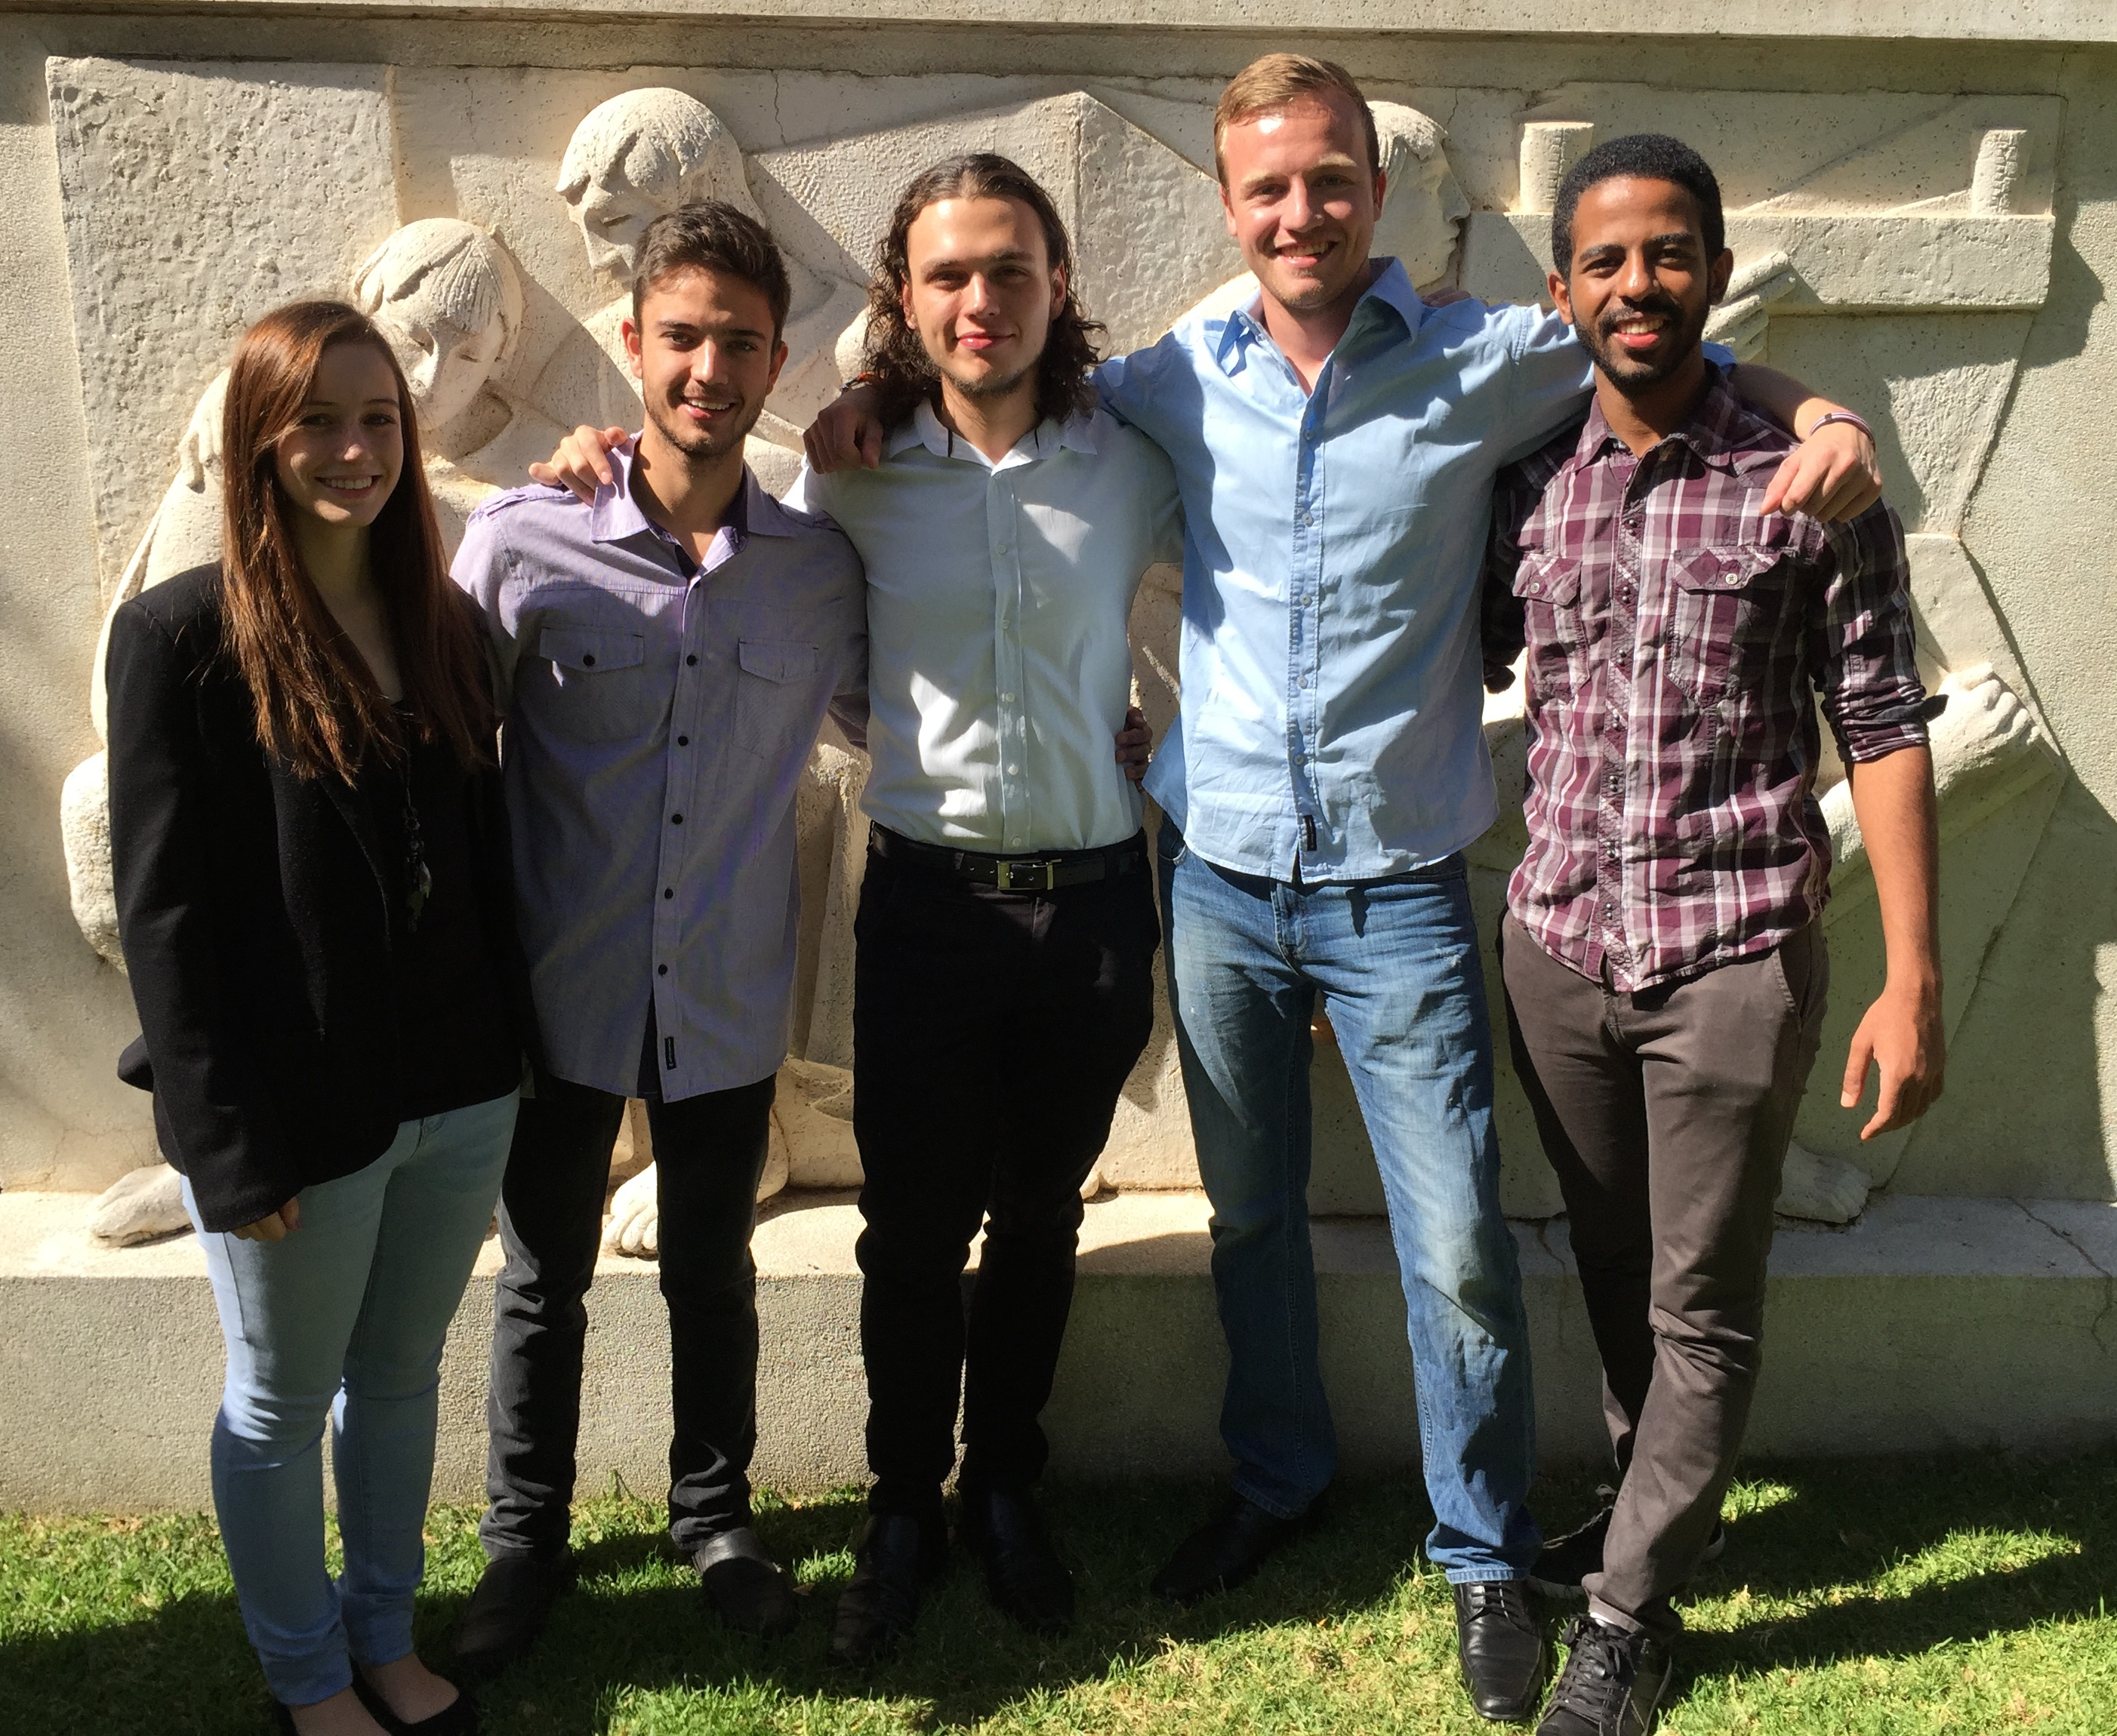
\includegraphics[scale=0.1]{group}}
\vspace*{2\baselineskip}

{\itshape The University of Pretoria \\ Computer Science Department\par} % Editor affiliation

\vfill 

\endgroup}

%Document starts here

\begin{document} 

\pagestyle{empty} % Removes page numbers

\titleGP % This command includes the title page



  % begin the content of the document
\sloppy  % this to relax whitespacing in favour of straight margins


% title on top of the document
\maintitle{Werner Mostert}{July 29,1994}{Last update on \today}

\nobreakvspace{0.3em}  % add some page break averse vertical spacing

\noindent\href{mailto:werner.dot.mostert1.at.gmail.dot.com}{werner.mostert1\mbox{}@\mbox{}gmail.com}\sbull
\textsmaller{+}27.713618606\sbull
\href{https://za.linkedin.com/pub/werner-mostert/99/341/258}{https://za.linkedin.com/pub/werner-mostert/99/341/258}
\\
2203 The Gables\sbull
1138 Prospect Street\sbull
Hatfield\sbull
Pretoria\\

\spacedhrule{0.9em}{-0.4em}  % a horizontal line with some vertical spacing before and after
\begin{center}
\roottitle{Summary}  % a root section title
\end{center}


\vspace{-1.3em}  % some vertical spacing
\begin{multicols}{3}% open a multicolumn environment

\noindent \fbox{
\includegraphics[width=\linewidth]{werner}}\\I am a very driven person with very clear goals in terms of my career as well as my personal life. I believe in honesty above all else and making a valuable contribution towards society. In my opinion, one of the greatest injustices that can be done by man, is refusing to pass on what one has learnt and experienced, for without this happening there can be no progress. My dream is to be remembered for the feats that I had accomplished in my lifetime. I am extremely passionate about technology, specifically software development, which is the reason why I chose to study Computer Science at a tertiary level. I am particularly fond of new challenges that test my abilities allowing for growth, self-improvement and the improvement of others. My family and friends are an extremely important factor in my life and I would see them proud of the man that I am, and want to be. 

\end{multicols}

\spacedhrule{0em}{-0.4em}

\roottitle{Experience}

\headedsection
  {\href{http://www.bbd.co.za}{Barone, Budge \& Dominick (Pty) Ltd}}
  {\textsc{Houghton Estate, Johannesburg}} {%
  \headedsubsection
    {Bursar}{Jan\apo15 -- present}
    {\bodytext{BBD implements and maintains complex business systems. A customer with a requirement for custom software, which must fit into their business, and must meet the business goals approaches BBD with the goal in mind of obtaining a software solution thereof.\\}}
    }
    
\headedsection
  {\href{http://www.bbd.co.za}{University of Pretoria, Computer Science Department}}
  {\textsc{Hatfield, Pretoria}} {%
  \headedsubsection
    {Teaching Assistant}{Jul\apo14 -- present}
    {\bodytext{As a teaching assistant for Data Structures and Algorithms, Netcentric Computer Systems and Software Modelling it is expected of one to have a good understanding of design patterns, general algorithm implementations and data structures in the Computer Science field as well as knowledge of web development and other networking related software development.\\}}
    }
    
\headedsection  % sets the header for the section and includes any subsections
  {\href{http://www.dvt.co.za}{Dynamic Visual Technologies}}
  {\textsc{Hyde Park, Johannesburg}} {%
  \headedsubsection
    {Junior Software Developer}
    {Nov \apo14 -- Jan\apo15}
    {\bodytext{DVT is a software development and related services business. They build, implement and support software, and  provide those services that ensure business concepts are clear, that practical needs are met, and that software is written to specifications. \\}}
}
    
\spacedhrule{-0.2em}{-0.4em}


\roottitle{Technical Skills}

\inlineheadsection  % special section that has an inline header with a 'hanging' paragraph
  {Technical expertise:}
  {Software design and implementation. Big fan of Agile methodologies. I regularly utilise Java/\nsp \CPP, yet flirts regularly with C\#.  Proper knowledge of web technologies:\ \acr{HTML+CSS}, \acr{XML},  \acr{REST}, \acr{.NET}, and JavaScript (including WebGL). Elementary knowledge of Artificial Intelligence related methods, such as optimisation problems.}

\vspace{0.5em}
\inlineheadsection
  {Natural languages:}
  {Afrikaans \emph{(mother tongue)}, English \emph{(full professional proficiency)}, French \emph{(elementary proficiency)}.}


\spacedhrule{1.6em}{-0.4em}

\roottitle{Interests}
\inlineheadsection
  {Non-exhaustive:}
  {Online gaming, running, music, reading, travel, foreign cultures, most things French related, cooking, open source movements, software development.}

  
\spacedhrule{1.6em}{-0.4em}  
  
\roottitle{Non - Technical Strengths}

\inlineheadsection
  {Social skills:}
  {I believe myself to be a rather "likeable" person, meaning I am very seldom found to be antagonistic towards others. I am a people person. I enjoy meeting and spending time with new and interesting people.}
  
\inlineheadsection
  {Professional skills:}
  {In a professional working environment I strive to be a very punctual, concise and informed individual. My approach towards professionalism relies on the concepts of honesty, determination, perseverance and most of all proper communication.}
  
\spacedhrule{1.6em}{-0.4em}  
  
\roottitle{Why DVT Drive Stats?}

\inlineheadsection
  {Because:}
  {I am very interested in mobile development, particularly for Android devices. I feel this project is very applicable to modern day life and can actually make a difference in people's lives. As a result of my previous experience with DVT, I will always jump to the opportunity to engage with the people and company.}


  % begin the content of the document
\sloppy  % this to relax whitespacing in favour of straight margins


% title on top of the document
\maintitle{Michelle Swnepoel}{February 1,1994}{Last update on \today}

\nobreakvspace{0.3em}  % add some page break averse vertical spacing

\noindent\href{mailto:michelle4swanepoel.at.gmail.dot.com}{michelle4swanepoel\mbox{}@\mbox{}gmail.com}\sbull
\textsmaller{+}27.836452606
\\
10 Shamrock Street\sbull
Ferndale Ext 3\sbull
Randburg

\spacedhrule{0.9em}{-0.4em}  % a horizontal line with some vertical spacing before and after
\begin{center}
\roottitle{Summary}  % a root section title
\end{center}


\vspace{-1.3em}  % some vertical spacing
\begin{multicols}{3}% open a multicolumn environment

\noindent 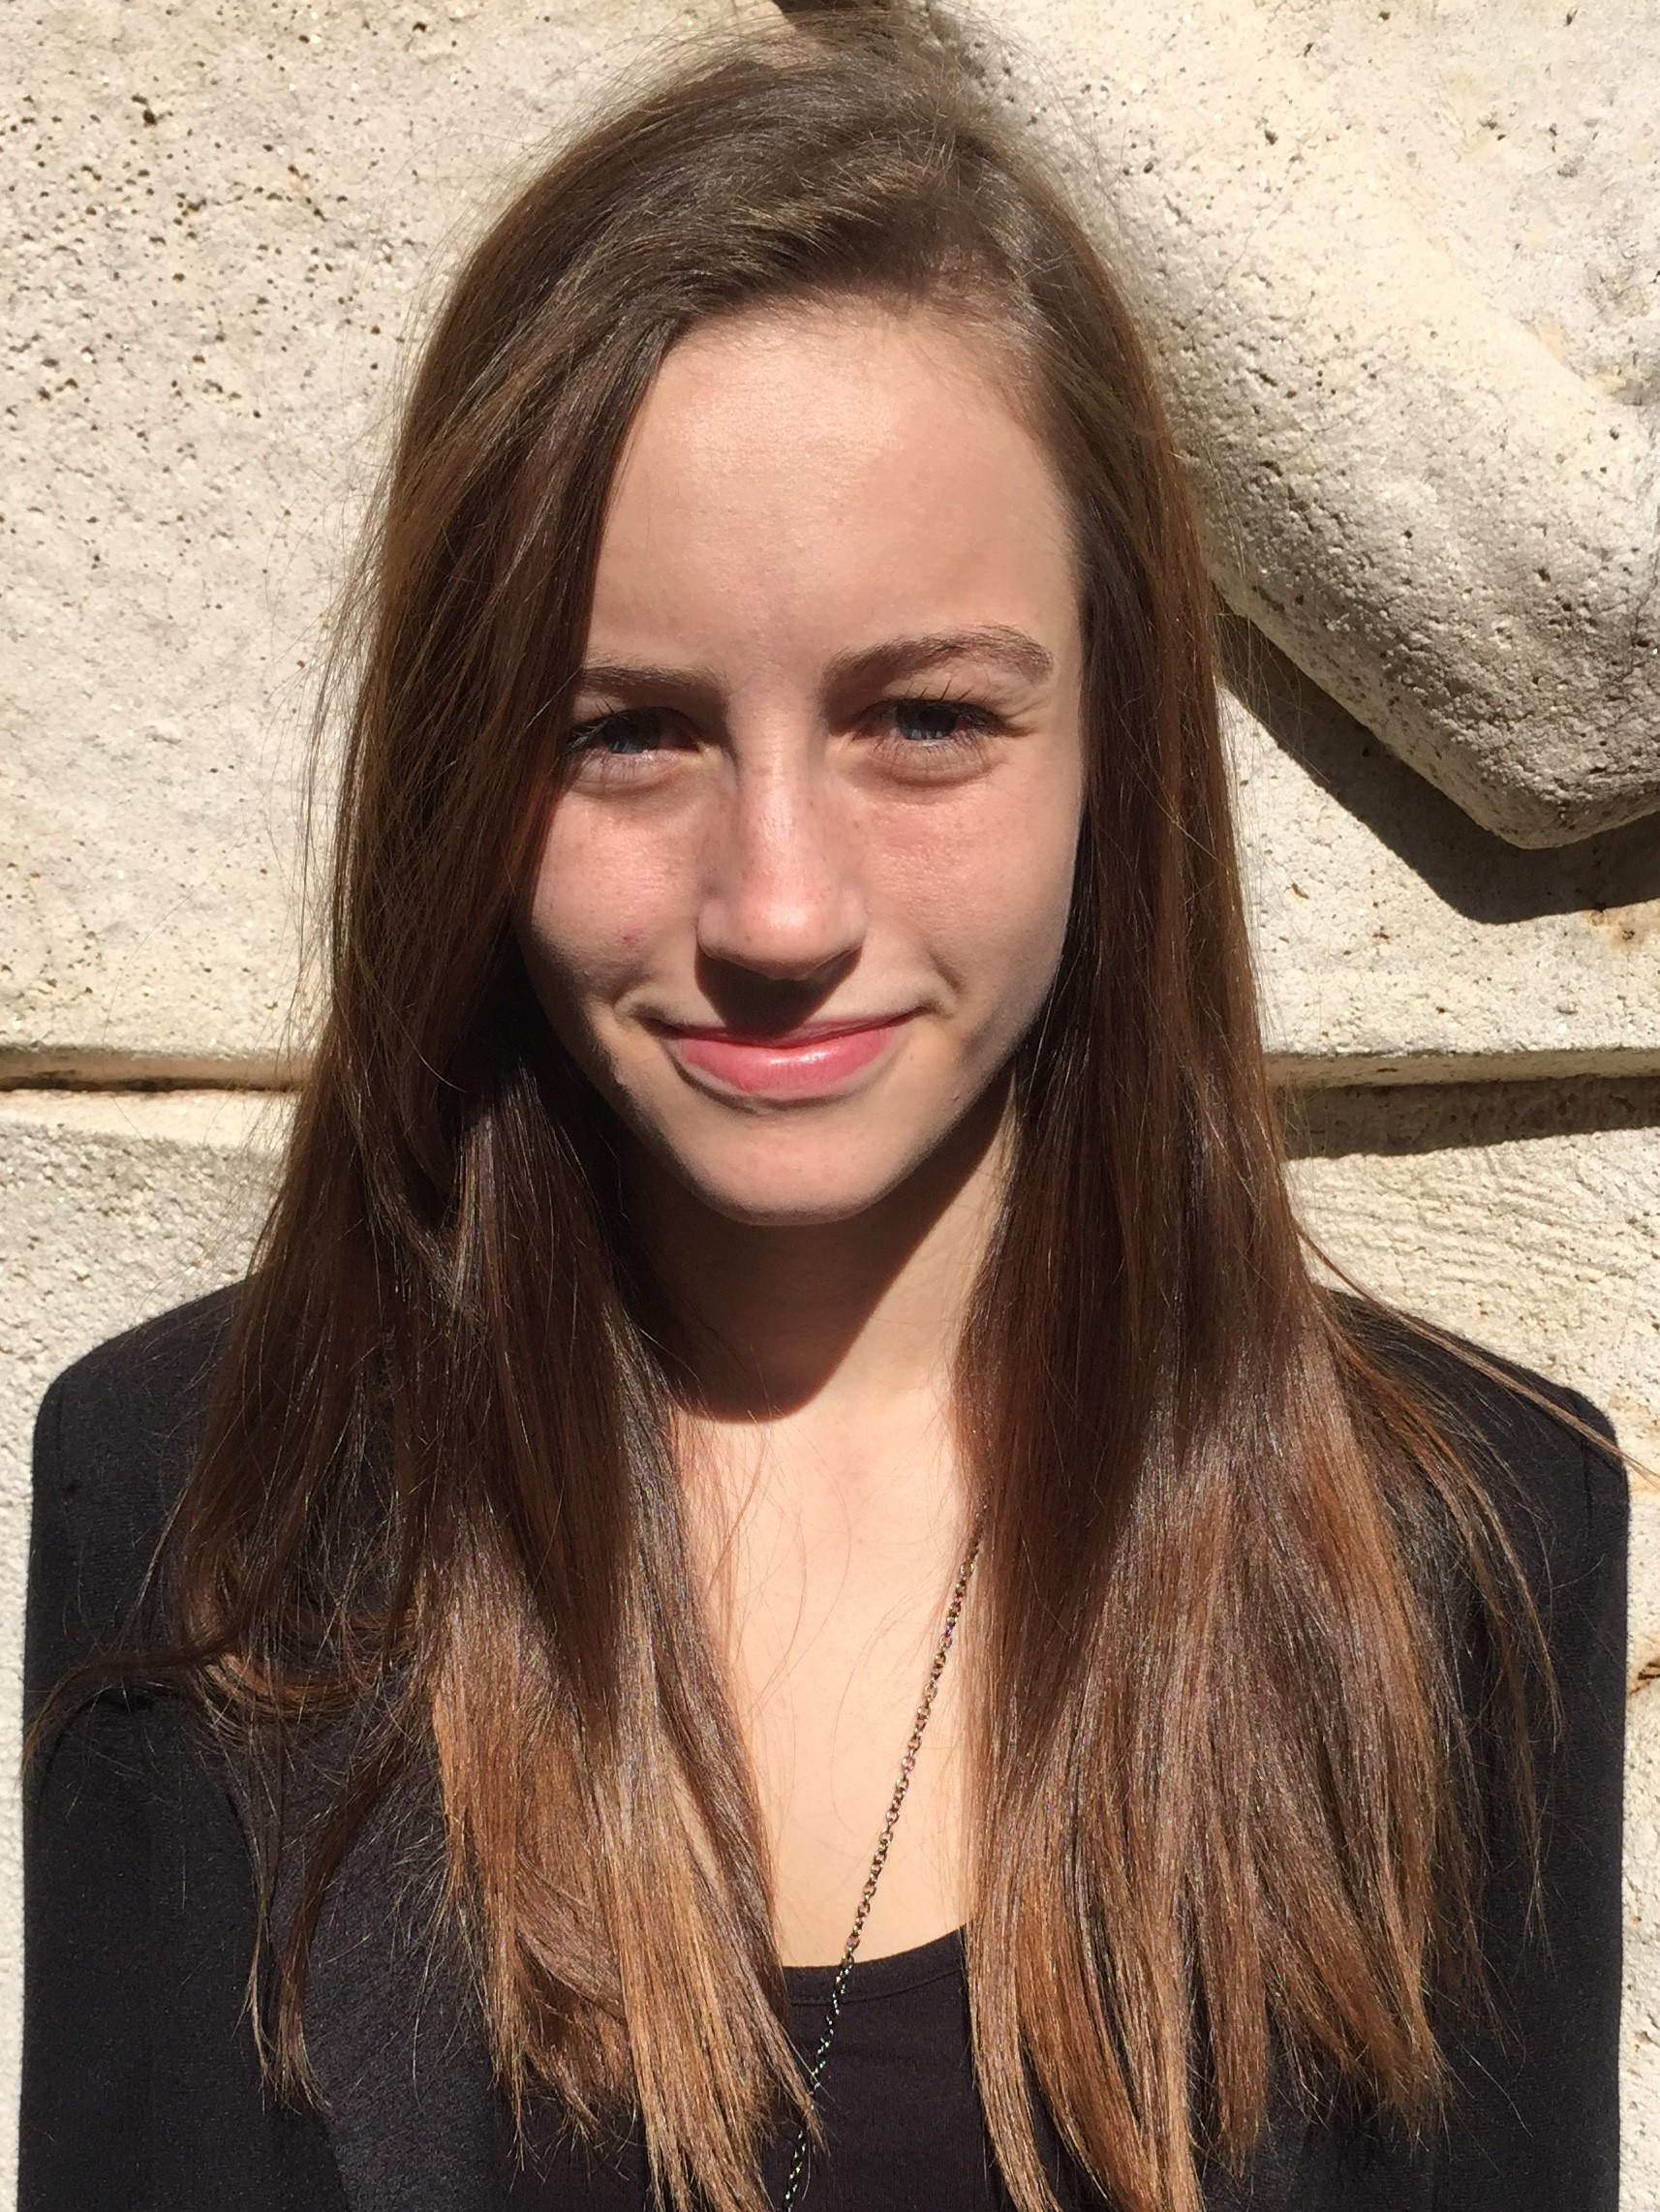
\includegraphics[width=\linewidth]{michelle}\\I see myself as a person who is invested in my personal growth in all aspects of my life. I am currently double majoring in Computer Science and am still deciding whether I want to do my honours degree next year or start working.  When I feel everything around me is going to fast and that I need a getaway, I will most definitely grab the book I'm currently reading and enjoy a few pages. I also enjoy watching series, building puzzle and playing 30 Seconds with my mom and sister - and always  a cup of coffee. One of my other passions in life is dogs and animals in general. Close friends and family see me as a person who is diligent, respectful, sincere, modest and compassionate. I am an introvert, but enjoy observing and getting to know new people. I get my energy by accomplishing something that I had to work hard for and working with people.


\end{multicols}

\spacedhrule{0em}{-0.4em}

\roottitle{Experience}

    
\headedsection
  {\href{http://www.up.ac.za}{University of Pretoria, Computer Science Department}}
  {\textsc{Hatfield, Pretoria}} {%
  \headedsubsection
    {Teaching Assistant}{Feb\apo14 -- Jul\apo14 and Feb\apo15 -- present}
    {\bodytext{I was a teaching assistant for a Introduction to Computer Science module, where it is needed to understand some
	basic concepts underlying computer science. I am now a teaching assistant for Data Structures and Algorithm, which requires 	the understanding of advanced data structures.\\}}
    }
        
\spacedhrule{-0.2em}{-0.4em}


\roottitle{Technical Skills}

\inlineheadsection  % special section that has an inline header with a 'hanging' paragraph
  {Technical expertise:}
  {Java, C/C++, assembly, CSS, HTML, JavaScript (also WebGL), XML, PHP, AJAX and jQuery}

\vspace{0.5em}
\inlineheadsection
  {Natural languages:}
  {Afrikaans \emph{(home language)}, English.}

\spacedhrule{1.6em}{-0.4em}  

\roottitle{Interests}
\inlineheadsection
  {Non-exhaustive:}
  {I enjoy reading books, mostly fiction. Spending time with my family and friends is one of my favourite activities and also to 		go to new places to explore. The human way of living interests me and I enjoy reading up on it.}

\spacedhrule{1.6em}{-0.4em}  
  
\roottitle{Non - Technical Strengths}

%\inlineheadsection
I consider myself as someone with good communications skills, enjoying it to work with people. I will always be open to new experiences and opportunities. Honesty is important to me, thus I will always be be open and trustworthy. I am also someone who grasps a new topic quite quickly. These strengths are propagated throughout my social and professional life.
   
\spacedhrule{1.6em}{-0.4em}  
  
\roottitle{Why CSIR Eaves Dropping Protection?}

\inlineheadsection
  {Because:}
  {When I read the project proposal for the first time, the idea immediately jumped out to me. It sounds like a fun project to do as a team and something we can be proud of afterwards. Even though the project will challenge me and I will have to learn some new technologies and skills, it sounds still within in reach for us as a team to accomplish. }
%

  % begin the content of the document
\sloppy  % this to relax whitespacing in favour of straight margins



% title on top of the document
\maintitle{Kale-ab Tessera}{December 8,1994}{Last update on \today}

\nobreakvspace{0.3em}  % add some page break averse vertical spacing

\noindent\href{mailto:kaleabtessera.at.gmail.dot.com}{kaleabtessera\mbox{}@\mbox{}gmail.com}\sbull
\textsmaller{+}27.766806878\sbull
\\
House Boekenhout\sbull
LC de Villiers Campust\sbull
Hatfield\sbull
Pretoria\\

\spacedhrule{0.9em}{-0.4em}  % a horizontal line with some vertical spacing before and after
\begin{center}
\roottitle{Summary}  % a root section title
\end{center}


\vspace{-1.3em}  % some vertical spacing
\begin{multicols}{3}% open a multicolumn environment

\noindent 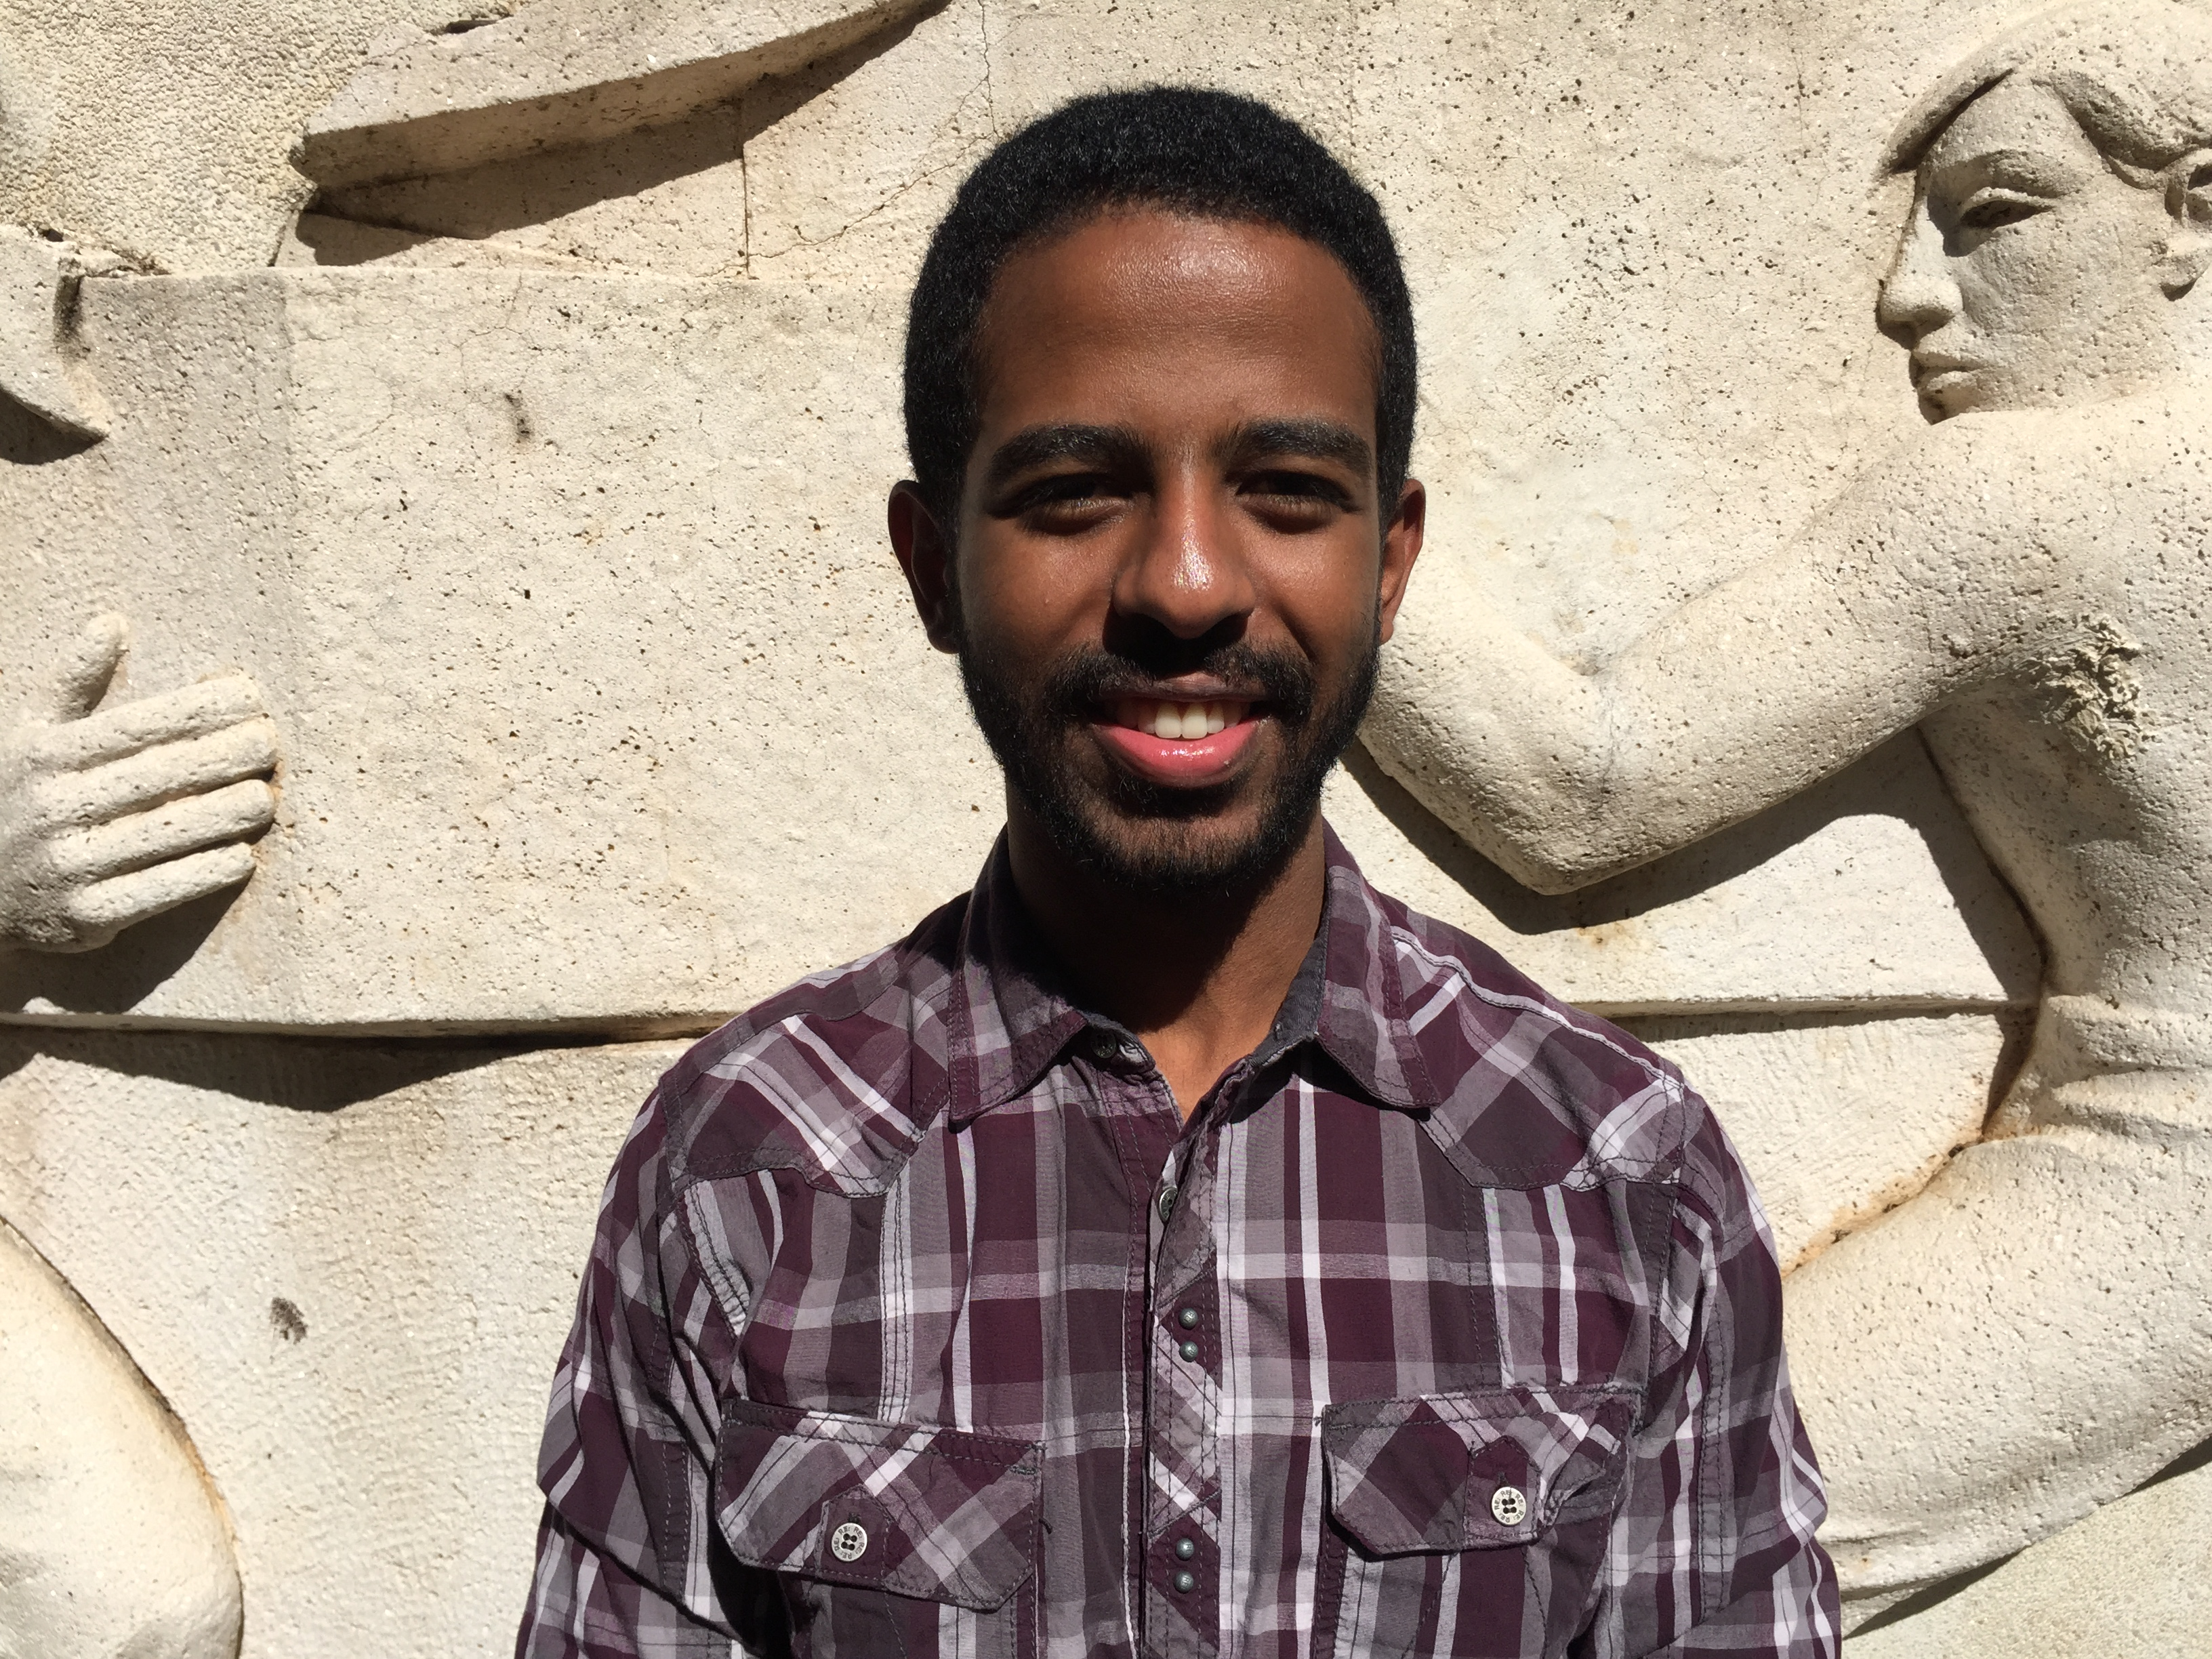
\includegraphics[width=\linewidth]{kaleab}\\Ambitious programmer with strong leadership and relationship skills. Adaptable and very open to learning new programming languages and methodologies, in order to build on previous knowledge. Hardworking yet still innovative. I try to live a live with as many experiences as possible cause I believe we can only learn and grow from things that challenge us. I am uncomfortable in my comfort zone. 

\end{multicols}

\spacedhrule{0em}{-0.4em}

\roottitle{Experience}
\headedsection  % sets the header for the section and includes any subsections
  {\href{http://www.cs.up.ac.za}{University of Pretoria, Computer Science Department}}
  {\textsc{Hatfield, Pretoria}} {%
  \headedsubsection
    {Teaching Assistant - COS 110}{july14 -- dec 14}
    {\bodytext{As a teaching assistant for Program design and Programming techniques good knowledge of 
 object-oriented (OO) programming. Concepts including inheritance and multiple inheritance, polymorphism, operator overloading, memory management (static and dynamic binding), interfaces and  encapsulation.\\}}
    }
    
\headedsection  % sets the header for the section and includes any subsections
  {\href{http://www.cs.up.ac.za}{University of Pretoria, Computer Science Department}}
  {\textsc{Hatfield, Pretoria}} {%
  \headedsubsection
    {Teaching Assistant - COS 212}{feb 14 --  present}
    {\bodytext{As a teaching assistant for Data Structures and Algorithms it was crucial to identify and recognise all the classical data structures; implement them in different ways; know how to measure the efficiency of implementations and algorithms; and have
further developed their programming skills, especially with recursion and polymorphism.\\}}
    }
    
\headedsection  % sets the header for the section and includes any subsections
  {\href{http://www.up.ac.za/boekenhout}{Boekenhout Res}}
  {\textsc{Hyde Park, Johannesburg}} {%
  \headedsubsection
    {House Committee Member, Secretary, Head of IT and Communications   }
    {aug 14 – present}
    {\bodytext{Helped lead various res students and mentored those with difficulties. I was also expected to solve technical 
dificulties such as problems connecting to the internet and also managing of social media. \\}}
}
    
\spacedhrule{-0.2em}{-0.4em}


\roottitle{Technical Skills}

\inlineheadsection  % special section that has an inline header with a 'hanging' paragraph
  {Technical expertise:}
  {Proficient in Java, C++ and html. Experience with Assembly ,C, sql and delphi. Well-equipped in data structures and algorithms}

\vspace{0.5em}
\inlineheadsection
  {Natural languages:}
  {English \emph{(full professional proficiency)}}


\spacedhrule{1.6em}{-0.4em}

\roottitle{Interests}
\inlineheadsection
  {Non-exhaustive:}
  {Keeping fir, playing tennis and soccer, dancing, cooking, technology trends , music, foreign cultures, software development and application of artificial intelligence}

  
\spacedhrule{1.6em}{-0.4em}  
  
\roottitle{Non - Technical Strengths}

\inlineheadsection
  {Social skills:}
  {I believe I am a born-leader and this has resulted in various leadership positions whether it be highschool, residence or the university. I am also quite easy to get along with due to my friendlyness and communication skills.}
  
\inlineheadsection
  {Professional skills:}
  {In a professional working environment I am self-driven and willing to work as hard as is required. I also strive to be very respectful,punctual and diligent in anything that I do.}
  
\spacedhrule{1.6em}{-0.4em}  
  
\roottitle{Why CSIR Ironman Image Throw Thingy?}

\inlineheadsection
  {Because:}
  {Not only am I interested in the obvious visual factors of this project, I am also interested in incorporating various technologies together. This project will be a challenge, but a rewarding one. Once completed, it will be used lecturers. Students and even for recreational purposes like watching movies. I want to be involved in working with software which has so much to offer the world. }
%  % begin the content of the document
\sloppy  % this to relax whitespacing in favour of straight margins


% title on top of the document
\maintitle{Keagan Thompson}{April 16, 1994}{Last update on \today}

\nobreakvspace{0.3em}  % add some page break averse vertical spacing

\noindent\href{mailto:u13023782.at.gmail.dot.com}{u13023782\mbox{}@\mbox{}gmail.com}\sbull
\textsmaller{+}27.822182880\sbull
\\
216 The Circuits\sbull
1228 Prospect Street\sbull
Hatfield\sbull
Pretoria\\

\spacedhrule{0.9em}{-0.4em}  % a horizontal line with some vertical spacing before and after
\begin{center}
\roottitle{Summary}  % a root section title
\end{center}


\vspace{-1.3em}  % some vertical spacing
\begin{multicols}{3}% open a multicolumn environment

\noindent 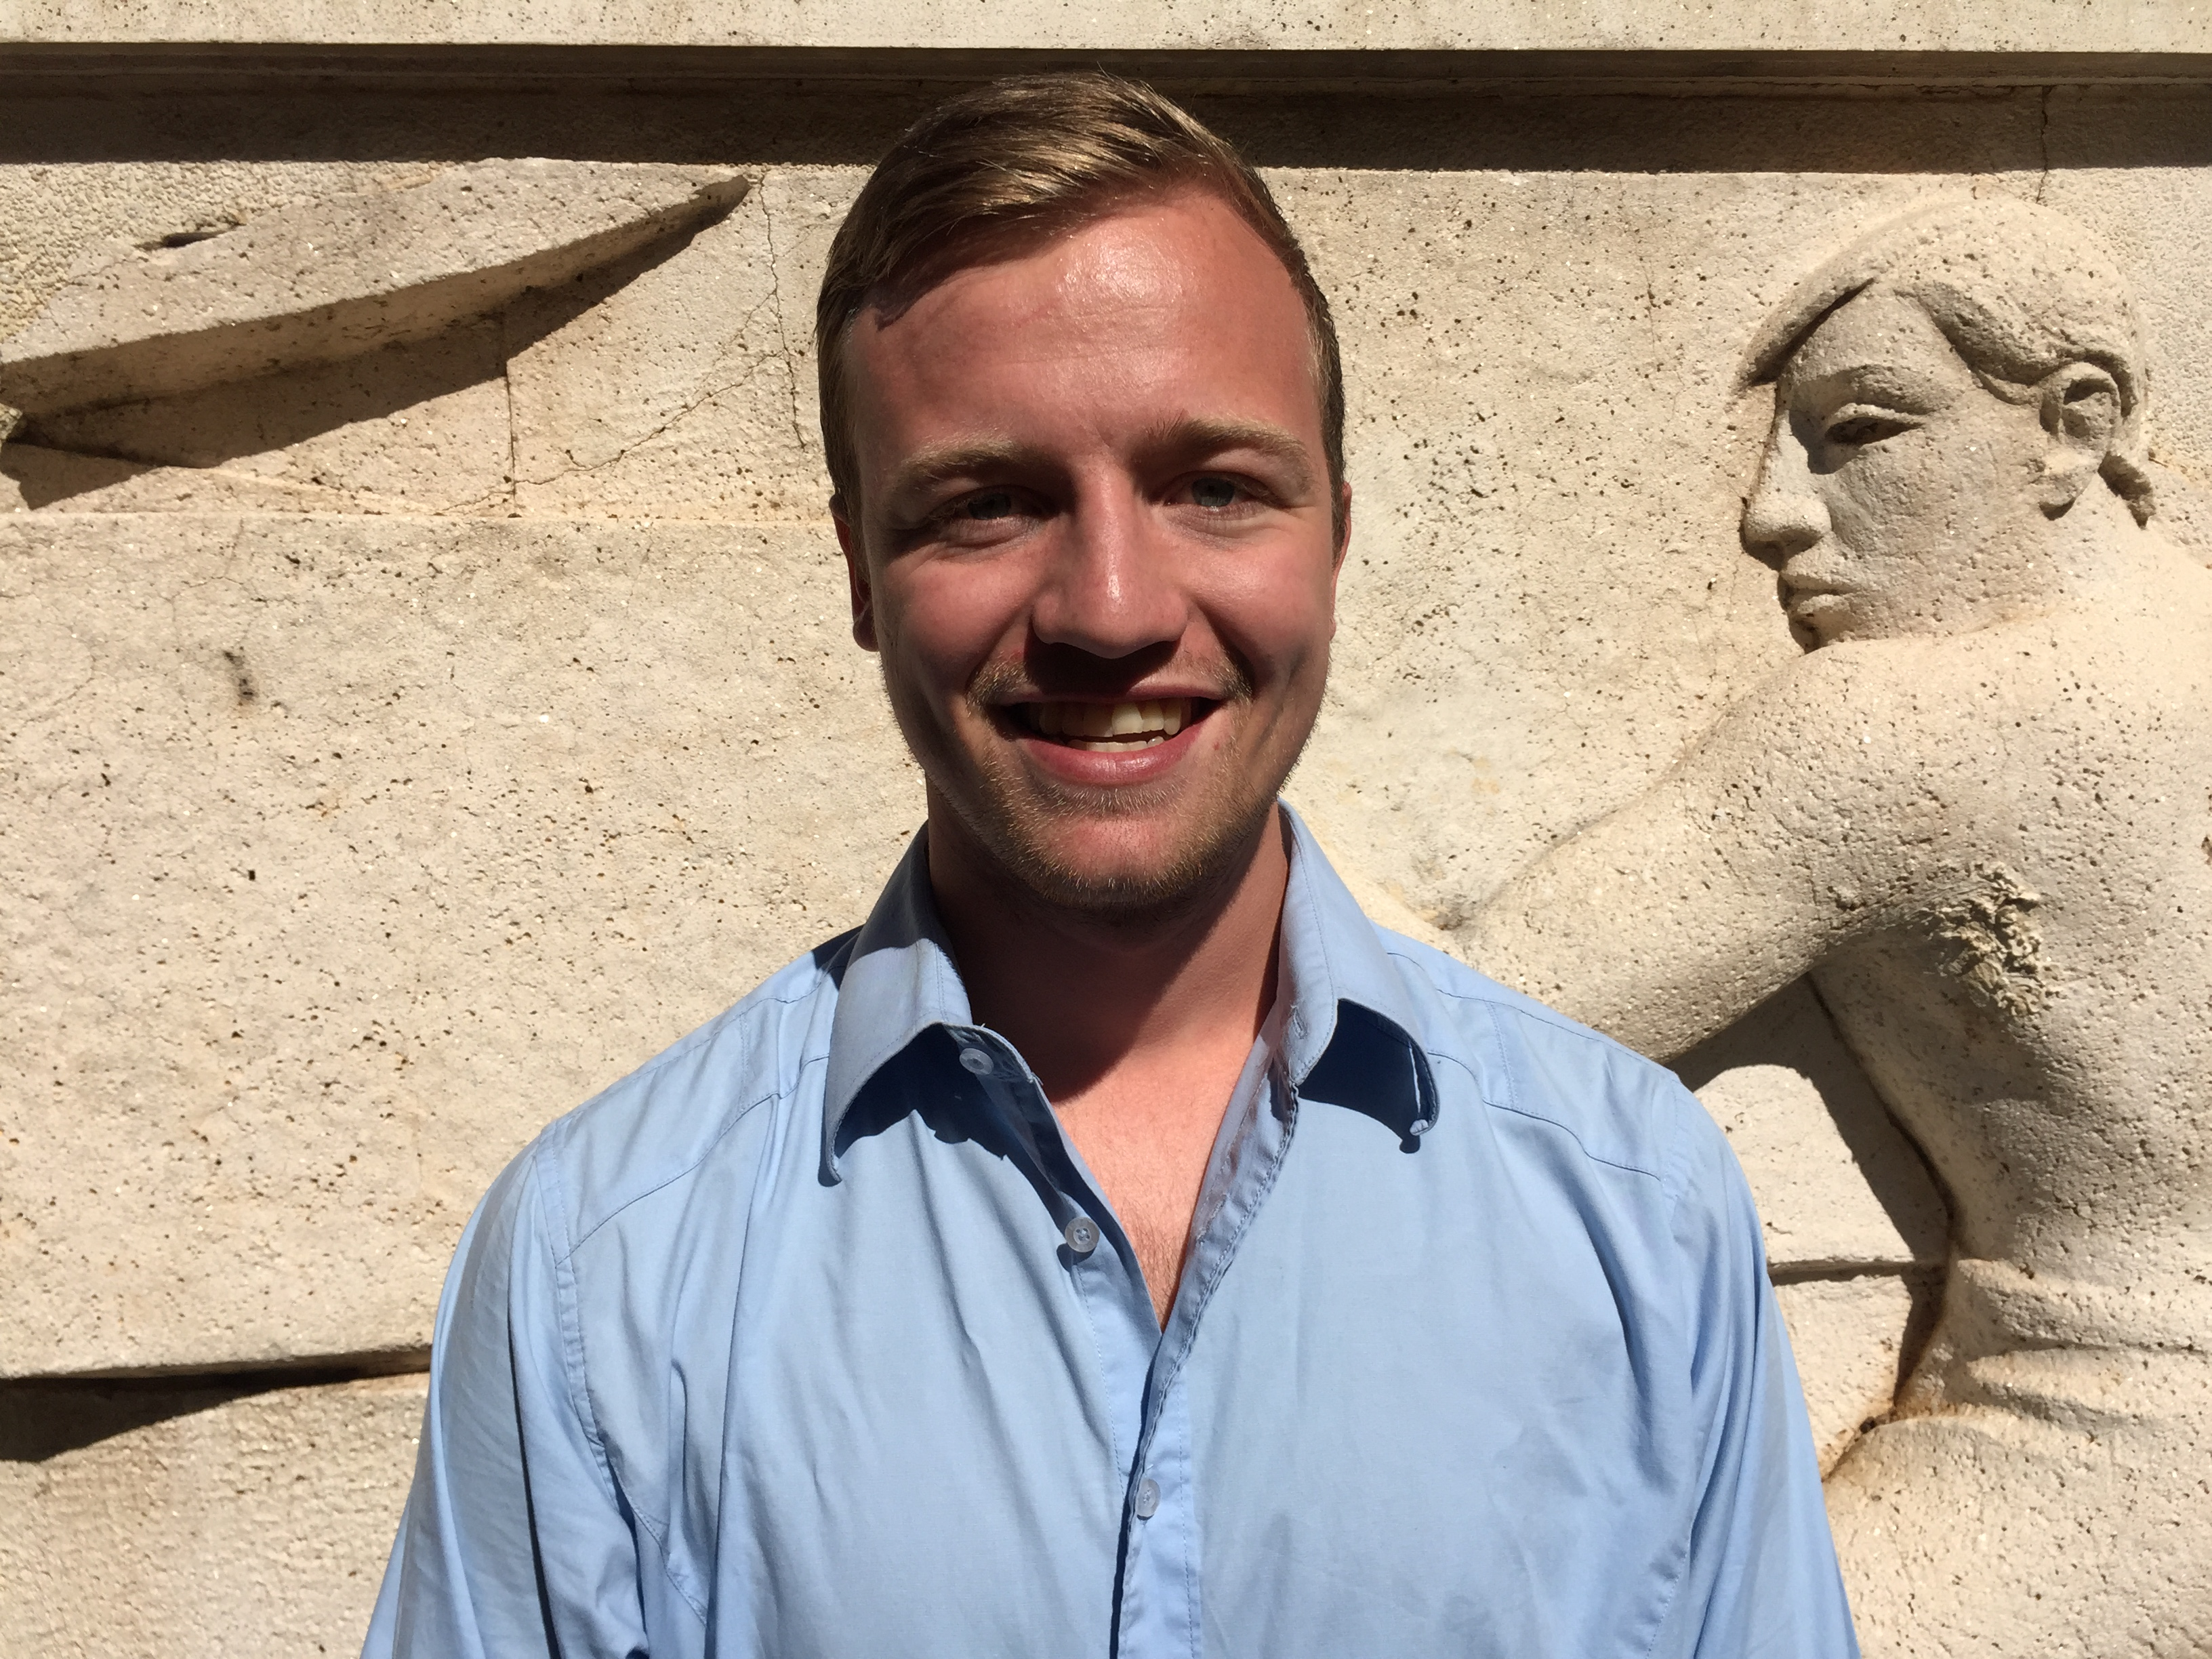
\includegraphics[width=\linewidth]{keagan}\\I am first and foremost career-driven. My primary aspirations in life are reaching for the highest branches of my career and having a healthy family lifestyle. While enjoying all aspects of life as a student, I still strive to always consider my future successes in society and the impact that any actions I commit may have on others as a result. Whilst acknowledging that it is necessary to help others to the best of my ability in advancing their own lives, I take a larger interest in ensuring a secure, comfortable lifestyle for myself. The technological environment has captivated my interest from a very young age and my fixation on developing technology that will help the human race in experiencing a more enjoyable life is a testament to that. It is through software development that I hope to leave my legacy in this world, since I see this as the most effective way for myself to leave this world in a better state than I found it. I am eager to tackle new challenges and pride myself on the fact that I am always able to find a solution to a problem. It is for this reason that I can describe my approach to programming using the expression "Where there is a will, there is a way". Although I am confident of my abilities as a software developer, I respect the fact that there are people who have a much broader knowledge of the field than I do and am willing to learn from these people in order to further my own experience.
\end{multicols}

\spacedhrule{0em}{-0.4em}

\roottitle{Experience}

\headedsection
  {\href{http://www.bbd.co.za}{Barone, Budge \& Dominick (Pty) Ltd}}
  {\textsc{Houghton Estate, Johannesburg}} {%
  \headedsubsection
    {Bursar}{Jan\apo13 -- present}
    {\bodytext{BBD implements and maintains complex business systems. A customer with a requirement for custom software, which must fit into their business, and must meet the business goals approaches BBD with the goal in mind of obtaining a software solution thereof.\\}}
    }
    
\spacedhrule{-0.2em}{-0.4em}


\roottitle{Technical Skills}

\inlineheadsection  % special section that has an inline header with a 'hanging' paragraph
  {Technical expertise:}
  {Software development aspects including software design patterns, data algorithms and programming fundamentals (Novice). I have experience in Delphi (4 years), Java (3 years), C\# (3 years), C++ (1 year) and SQL (2 years).  I also have a wealth of experience with web technologies such as \acr{HTML}, \acr{XML}, and JavaScript (Angular, NodeJS, BootStrap, jQuery). Additionally, I have a moderate knowledge of various Artificial Intelligence concepts and an extensive experience in Information System modelling.}

\vspace{0.5em}
\inlineheadsection
  {Natural languages:}
  {English \emph{(mother tongue)}, Afrikaans \emph{(full professional proficiency)}, Greek \emph{(elementary proficiency)}.}


\spacedhrule{1.6em}{-0.4em}

\roottitle{Interests}
\inlineheadsection
  {Non-exhaustive:}
  {Technology, Sports (Rugby), Socialising, Outdoors, Gaming, Travelling}

  
\spacedhrule{1.6em}{-0.4em}  
  
\roottitle{Non - Technical Strengths}

\inlineheadsection
  {Social skills:}
  {I am a person who has a witty sense of humour. I see myself as the forerunner of my group of friends and am always keen to organise a get-together at my place of residence. In terms of meeting new people, I portray my true self because I believe in always being who I am, and I have been in contact with many different kinds of people so I have a good understanding of communication with most people.}
\inlineheadsection
  {Professional skills:}
  {I always try my best to be punctual and to have work completed by the deadline as this is the only way a group will be able to complete a project effectively and I like to consider actions carefully in conflict situations rather than force my own ideas upon others.}
  
\spacedhrule{1.6em}{-0.4em}  
  
\roottitle{Why CSIR Eaves Dropping Protection?}

\inlineheadsection
  {Because:}
  {For every person involved in IT, malware is a dark interest. I have always been interested in creating malware but only to be able to help people understand how to avoid it. I also want to learn more about mobile app development and so I see this project as a good opportunity to broaden my knowledge within the software development sector, and also to create a product that very well could become useful to businesses around the world.}

\section{Project Execution}
\subsection{Development Methodology}
In order to ensure that we meet the client's requirements and expectations to deliver a satisfactory product we intend to follow the Agile Development Methodology. We believe that this methodology aids the client in clearly  communicating the vision of the project and it will help us as developers to quickly respond to problems that the client, or we, identify. 
\input{communicationTechnologies}
\subsection{Ideas and Technologies}
\subsubsection{Technologies to be Used}
After due consideration and taking into account the received requirements, the following technologies will be used:
\begin{description}
	\item[ASP.NET MVC 5]\hfill\\
	%Description
	\item[ASP.NET Web API]\hfill\\
	
	\item[C\#]\hfill\\
	
	\item[MySQL]\hfill\\	
	
	\item[Xamarin]\hfill\\
	
	
\end{description}
	
\subsubsection{Implementation Ideas}	
In order to develop the back end of the system [API]

	
\subsubsection{Project Extension Ideas}
The following was considered as possible future extensions on the current project specifications:

\begin{itemize}
	\item Android watch notification sister-application\\
	The idea behind this is that while the main app is tracking the user's travelling speed, if it is the case that a user is travelling at a rate which is greater than the speed limit in his vicinity the user will be made aware of this fact. This alert can take place in the form of vibrations or sound emitted by the watch as to not interfere with the user's driving.
	
	\item 
\end{itemize}
%\newline
\subsection{Deliverables}
\small
\begin{enumerate}
\item Original Tender Document
\item Requirements Specification
\item Architecture and Design Document
\item Developer's Guide
\item All Source Code
\end{enumerate}



\end{document}